\documentclass[11pt]{article}
\usepackage{amsmath}
\usepackage{graphicx}
\usepackage{subfigure}
\graphicspath{ {fig/} }
\usepackage{pdfpages}
\usepackage{csvsimple}
\usepackage{float}
\usepackage{color}
\usepackage{comment}
\newcommand\Deq{\mathrel{\stackrel{\makebox[0pt]{\mbox{\normalfont\tiny D}}}{=}}}

\begin{document}
\section{Abstract}

In case of high-dimensional image data with intractable latent variable, we propose the Auto-Encoding Variational Bayes (AEVB) algorithm. AEVB is based on Auto-Encoding (a feedforward Multiple-Layer Perceptron algorithm for data compression) but with its optimization objective function replaced by Variational Bayes approach and implented by stochastic gradient descent (SGVB estimator). SGVB estimator achieves efficient approximation of the intractable posterior and likelihood inside Auto-Encoding and results in a successful dimension reduction AEVB algorithm for large image datasets.

We apply AEVB to the example of binary dataset MNIST and continuous variable dataset FreyFaces and achieves parameter estimation, dimension reduction and image reconstruction. We also compare different gradient methods inside AEVB to optimize the inference. Our code is in package:..............

\section{Background}
The Variantional Bayesian (VB) approach is to optimize an approximation to the intractable posterior. However, the common mean-field approach requires analytical solutions of expectation with respect to the approximate posterior which is also intractable in many cases. In this report, we introduce the Stochastic Gradient Variantional Bayes (SGVB) estimator which is used for an efficient approximation of the posterior  based on a reparameterizatio of the variational lower bound. The optimization process uses standard stochastic gradient ascent techniques. \\

To deal with image data, we propose the Auto-Encoding VB (AEVB) algorithm. AEVB is essentially a Auto-Encoding (feedforward Multiple-Layer Perceptron for data compression algrithom) with its optimization objective function replaced by Variational Bayes approach and implented by stochastic gradient descent. Using SGVB estimator in original Auto-Encoding algorithm optimizes a recognition model that allows us to efficiently approximate the posterior inference with ancestral sampling, which results in an efficient learning of the model parameters without costly iterative inference schemes (such as MCMC) per datapoint.\\

We refer to the paper of Kingma and Welling (2013) for the algorithm. We first describe the setting and the goals of the paper. \\
The dataset $X = \{x^{(i)}\}^N_{i=1}$ consists of $N$ i.i.d samples of some continuous or discrete variable $x$.  $z^{(i)}$ is a latent variable which $x^{(i)}$ depends on. The problem is: 
\begin{itemize}
\item The likelihood of $p_{\theta}(x|z)$ has a complicated form and thus the posterior of z,$p_{\theta}(z|x)$ is intractable. The marginal likelihood of x, $\int p_{\theta}(z)p_{\theta}(x|z)$ is intractable in this case too.

\item The dataset of $x$ can be very large and high dimensional, parameter estimation for $\theta$ using usual MCMC and EM could be too slow. A dimension reduction is preferrable.
\end{itemize}

In this scenerio, we want to achieve: 
\begin{itemize}
\item Efficient approximation of parameter ${\theta}$.
\item Efficient approximation of likelihood of latent variable $z$ and original high dimensional variable $x$.
\end{itemize}


\section{Algorithm}

\subsection{Variational Bayes and SGVB Estimators} 

We use the variational approximation $q_{\phi}(z|x)$ to approximate the intractable true posterior $p_{\theta}(z|x)$. The approximation parameter $\phi$ is learned jointly with $\theta$ in later steps. The likelihood of  $X = \{x^{(i)}\}^N_{i=1}$ $\log p_\theta(x^{(1)},...,x^{(N)})=\sum^N_{i=1}\log p_\theta(x^{(i)})$ can be rewritten as:

\begin{equation}
\log p_\theta(x^{(i)})=D_{KL}(q_\phi(z|x^{(i)})||p_\theta(z|x^{(i)}))+L(\theta, \phi; x^{(i)})
\end{equation}

where the first RHS term is the KL divergence of the approximate from the true posterior and it is non-negative. The second RHS term $L(\theta, \phi; x^{(i)})$ is the variational lower bound on the marginal likelihood of the datapoint $i$. Thus we have:

\begin{align}
\log p_\theta(x^{(i)}) &\geq L(\theta, \phi; x^{(i)})=E_{q_\phi(z|x)}[-\log q_\phi(z|x)+\log p_\theta(x,z)]\\
& =-D_{KL}(q_\phi(z|x^{(i)}))||p_\theta(z|x^{(i)}))+E_{q_\phi(z|x^{(i)})}[p_\theta(x^{(i)}|z)]
\end{align}


Instead of optimizing intractable $\log p_\theta(x^{(i)})$ , we equivalently optimize the lower bound $L(\theta, \phi; x^{(i)})$ w.r.t both the variational parameters $\phi$ and generative parameters $\theta$.

With any chosen $q_\phi(z|x)$, we reparameterize the random variable $\widetilde{z}\sim q_\phi(z|x)$, with an auxiliary noise $\epsilon$:

\begin{equation}
\widetilde{z}=g_\phi(\epsilon, x), \epsilon\sim p(\epsilon)
\end{equation}

Here we can form Monte Carlo estimates of expectations of some function $f(z)$ w.r.t $q_\phi(z|x)$ as follows:

\begin{eqnarray}
E_{q_\phi(z|x^{(i)})}[f(z)]=E_{p(\epsilon)}[f(g_\phi (\epsilon, x^{(i)}))]\simeq\frac{1}{L}\sum^L_{l=1}f(g_\phi (\epsilon^{(l)}, x^{(i)}))  \\
\epsilon^{(l)}\sim p(\epsilon)
\end{eqnarray}

We apply this technique to the variational lower bound and yield the generic SGVB estimator $\widetilde{L}^A(\theta, \phi; x^{(i)})\simeq L(\theta, \phi; x^{(i)})$:

\begin{eqnarray}
\widetilde{L}^A(\theta, \phi; x^{(i)})=\frac{1}{L}\sum^L_{l=1}\log p_\theta (x^{(i)}, z^{(i, l)})-\log q_\phi(z^{(i, l)}|x^{(i)})\\
z^{(i,l)}=g_\phi (\epsilon^{(i, l)}, x^{(i)})
\end{eqnarray}

When $D_{KL}(q_\phi(z|x^{(i)})||p_\theta(z|x^{(i)}))$ can be analytically integrated, we only need to estimate the expected reconstruction error $E_{q_\phi(z|x^{(i)})}[p_\theta(x^{(i)}|z)]$ by sampling. Thus we have the second version of the SGVB estimator $\widetilde{L}^B(\theta, \phi; x^{(i)})\simeq L(\theta, \phi; x^{(i)})$:

\begin{eqnarray}
\widetilde{L}^B(\theta, \phi; x^{(i)})=-D_{KL}(q_\phi(z|x^{(i)}))||p_\theta(z|x^{(i)}))+\frac{1}{L}\sum^L_{l=1}\log p_\theta (x^{(i)}|z^{(i, l)})\\
z^{(i,l)}=g_\phi (\epsilon^{(i, l)}, x^{(i)})
\end{eqnarray}

The KL-divergence term can be interpreted as regularizing $\phi$ and $\widetilde{L}^B(\theta, \phi; x^{(i)})$ typically has less variance than $\widetilde{L}^A(\theta, \phi; x^{(i)})$. In this case, since KL-Divergence is analytical, we use the $\widetilde{L}^B$ as our SGVB estimator. 

\subsection{Auto-Encoding}
Auto-encoding is widely used for dimension reduction and data compression for images. We first recall the traditional autoencoder architecture:
\begin{eqnarray}
\phi: X\to F \\
\psi: F\to X \\
\phi, \psi = \arg\min||X-(\psi\circ\phi) X||^2
\end{eqnarray}

In the simplest case with only one hidden layer, the first stage (encoder stage) of an autoencoding takes the input $x \in R^d$ that is then mapped to the latent code $z \in R^k$.

\begin{equation}
\mathbf{z}=f_{\phi}(\mathbf{Wx}+\mathbf{b})
\end{equation}

where $f_{\phi}$ is an element-wise activation function such as a sigmoid function or a rectified linear unit. $\mathbf {W}$ is the weight matrix and $\mathbf {b}$ is the bias vector. $\phi$ is the parameter we want to estimate depending on W and b\\ 

Second, the decoder stage of the auto-encoding maps $\mathbf {z} \in R^k$ to the reconstruction $\mathbf {x'} \in R^d $ as of the same shape as $\mathbf{x}$:

\begin{equation}
\mathbf{x'}=f'_{\theta}(\mathbf{W'z}+\mathbf{b'})
\end{equation}

where $\mathbf f'_{\theta} ,\mathbf {W'}$ and $\mathbf {b'}$ for the decoder may differ in general from the corresponding $\mathbf {f_{\phi}} ,\mathbf {W}$ and $\mathbf {b}$ for the encoder. $\theta$ is the parameter we want to estimate depending on W' and b'.\\ 

These two stages in autoencoding are traditionally trained to minimise reconstruction errors:

\begin{eqnarray}
\mathbf{L(x, x')} = ||\mathbf{x}-\mathbf{x'}||^2 = ||\mathbf{x}-f'_{\theta}(\mathbf{W'}(f_{\phi}(\mathbf{Wx+b}))+\mathbf{b'})||^2 \\
W,b,W',b' = argmin \quad L 
\end{eqnarray}


Now we change traditional auto-encoding by our VB approach and SGVB estimator to generate AEVB. In AEVB, we do not use the traditional reconstruction loss function (Equation 16). We see encoder (Equation (14)) as variational approximation of z on x, and see decoder (Equation (15)) as conditional likelihood of x on z. Instead of minimizing $\mathbf{L(x, x')}$ in Equation(16), we use SGVB estimator $\widetilde{L}^B$ to maximize the variational lower bound. Equation (16) and (17) thus becomes: 
\begin{eqnarray}
\widetilde{L}^B(\theta, \phi; x^{(i)})=-D_{KL}(f_\phi(z|x^{(i)}))||p_\theta(z|x^{(i)}))+\frac{1}{L}\sum^L_{l=1}\log f'_\theta (x^{(i)}|z^{(i, l)})\\
W,b,W',b' = argmax L  \quad updated-by-SGD
\end{eqnarray}


\subsection{AEVB (Auto-Encoding Variational Bayes) Algorithm}

Specifically in our AEVB,  we use a neural network for encoding and decoding in the above section. Let the prior over the latent variables be the centered isotropic multivariate Gaussian $p_\theta(\mathbf{z})=\mathcal{N}(\mathbf{z};\mathbf{0}, \mathbf{I})$. We assume the true (but intractable) posterior takes on a approximate Gaussian form with an approximately diagonal covariance. In this case, we can let the variational approximate posterior be a multivariate Gaussian with a diagonal covariance structure:

\begin{equation}
\log q_\phi(\mathbf{z}|\mathbf{x}^{(i)})=\log\mathcal{N}(\mathbf{z};\mathbf{\mu}^{(i)}, \mathbf{\sigma}^{2(i)}\mathbf{I})
\end{equation}

where the mean and s.d. of the approximate posterior, $\mathbf{\mu}^{(i)}$ and $\mathbf{\sigma}^{2(i)}$, are outputs of the encoding MLP (a fully-connected neural network with a single hidden layer), i.e. nonlinear functions of datapoint $x^{(i)}$ and the variational parameters $\phi$:

\begin{eqnarray}
\log q_\phi=\log\mathcal{N}(\mathbf{z}; \mathbf{\mu}, \mathbf{\sigma}^2\mathbf{I})\\
\mathbf{\mu}=\mathbf{W_1h}+\mathbf{b_1}\\
\log\mathbf{\sigma}^2=\mathbf{W_2h}+\mathbf{b_2}\\
\mathbf{h}=\tanh(\mathbf{W_3z}+\mathbf{b_3})
\end{eqnarray}



Then, we sample from the posterior $\mathbf{z}^{(i,l)}\sim q_\phi(\mathbf{z}|\mathbf{x}^{(i)})$ using $\mathbf{z}^{(i,l)}=g_\phi(\mathbf{x}^{(i)},\epsilon^{(l)})=\mu^{(i)}+\sigma^{(i)}\bigodot\epsilon^{(l)}$ where $\epsilon^{(l)}\sim\mathcal{N}(\mathbf{0},\mathbf{I})$. With $\bigodot$ we signify an element-wise product. Since both the prior $p_\theta(\mathbf{z})$ and $q_\phi(\mathbf{z}|\mathbf{x})$ are Gaussian, KL divergence are analytically solved and we use $\widetilde{L}^B$ with a solved KL divergence:
%\begin{equation}
%-D_{KL}(q_\phi(z|x^{(i)}))||p_\theta(z|x^{(i)}))=\frac{1}{2}\sum_{j=1}^J(1+\log((\sigma_j^{(i)})^2)-(\mu_j^{(i)})^2-(\sigma_j^{(i)})^2)
%\end{equation}

\begin{equation}
L(\theta, \phi; \mathbf{x}^{(i)})\simeq\frac{1}{2}\sum_{j=1}^J(1+\log((\sigma_j^{(i)})^2)-(\mu_j^{(i)})^2-(\sigma_j^{(i)})^2)+\frac{1}{L}\sum_{l=1}^{L}\log p_\theta(\mathbf{x}^{(i)}|\mathbf{z}^{(i,l)})
\end{equation}

\textbf{Case 1: Binary Dataset (Binary Decoder)}\\
For binary dataset such as MNIST with N datapoints, we use a Bernoulli decoder for $\log p_\theta(\mathbf{x}^{(i)}|\mathbf{z}^{(i,l)})$:
\begin{eqnarray}
\log p_{\theta}(x|z) =\sum_{i=1}^N x_i \log y_i + (1-x_i)\cdot\log (1-y_i)\\
y=f_{sigmoid}(\mathbf{W_5}tanh(\mathbf{W_4}z+\mathbf{b_4})+\mathbf{b_5})
\end{eqnarray}
where $f_{sigmoid}$ is the sigmoid activation function.\\

\textbf{Case 2: Continuous Dataset (Gaussian Decoder)}\\
For datasets with continuous variables such as FreyFaces, we use the Gaussian decoder for $\log p_\theta(\mathbf{x}^{(i)}|\mathbf{z}^{(i,l)})$:

\begin{eqnarray}
\log p_\theta(x|z)=\log\mathcal{N}(\mathbf{x}; \mathbf{\mu}', \mathbf{\sigma}'^2\mathbf{I})\\
\mathbf{\mu}'=\mathbf{W_4h'}+\mathbf{b_4}\\
\log\mathbf{\sigma}'^2=\mathbf{W_5h'}+\mathbf{b_5}\\
\mathbf{h'}=\tanh(\mathbf{W_6x}+\mathbf{b_6})
\end{eqnarray}

$\{\mathbf{W}_i, \mathbf{b}_i\}$ are the weights and biases of the MLPs for encoder and decoder and the parameters that are actually updated and optimized in coding process. $\mathbf{\phi}=\{\mu, \sigma\}$ and $\mathbf{\theta}=y$ (Bernoulli) or $\mathbf{\theta}=\{\mu', \sigma'\}$ (Gaussian) are parameters we want to estimate as a result.

\section{Implementation}
Considering the size of the datasets, we run the model on each minibatch of size 100 and run 10000 epochs on Bernoulli case (MNIST) and 100000 epochs on Gaussian case (FreyFaces) with first 1000 burn-in. \\

Initializing Specific settings for the MNIST and Frey Face datasets: 
\begin{itemize}
\item The size of minibatch $M=100$ and the size of samples per datapoint $L=1$.
\item The initialized values of parameters $\phi_0$ and $\theta_0$ are randomly sampled from $\mathcal{N}(0,0.01)$.
\item Stepsizes used for updating parameters within the algorithm are adapted by Adagrad with parameters chosen from $\{0.01, 0.02, 0.1\}$.
\item When obtaining the likelihood lower bound, we trained the encoder and decoder with 100 hidden units for both MNIST, and Frey Faces dataset.
\end{itemize}

The steps of implementation can be summarized as: 

- Initialize parameters $\mathbf{\theta_0, \phi_0}$ 

- $\textbf{repeat}$:  

1. Draw a random minibatch of M datapoints from datasets of size N, noted as $X^M$ 

2. - Encoding: $X\to Z; q_{\phi}(z|x)$ 

   \quad - sample z from $q_{\phi}(z|x)$ with noise $\epsilon \sim \mathcal{N}(0,\mathcal{I})$ 
   
   \quad - Decoding: $Z\to X; p_{\theta}(x|z) $ 
   
   \quad - Note: $\theta$ and $\phi$ are jointly updated with objective function $L(\theta, \phi; \mathbf{x}^{(i)})$ in Equation(25) with Gradient Descent.

$\textbf{until}$: convergence of parameters ($\mathbf{\theta, \phi}$) or max-epochs is reached.

$\textbf{return}$: $\mathbf{\theta, \phi}$

We run the process above to get the estimation for $\mathbf{\theta, \phi}$ from the training set, and we test the estimations on the test set and reconstruct the images from both MNIST and FreyFaces. 

The complete code is done in python and in package : 


\section{Result}
\subsection{Convergence Analysis}
We operated the model on binary dataset(MNIST, dimension of $70000*28*28$)and continuous dataset (FreyFaces, $1965*28*20$). For MNIST, we used the first 60000 data points as training set, last 10000 as test set; and ran the Berboulli case AEVB with $10^5$ epochs. For FreyFaces, we used first 1500 data points as training, last 465 as testing; and ran  the Gaussian case AEVB with $10^6$ epochs with first 1000 burn-in. We repeated the model with latent variable $z$ of dimension $N_z= 2,3,5,10$ and plot the variational lower bound as below:

\begin{figure}[H]
\begin{center}
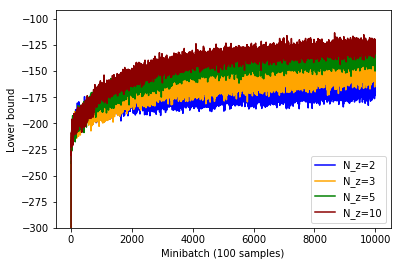
\includegraphics[width = 0.45\textwidth]{fig/Bernoulli_lb}
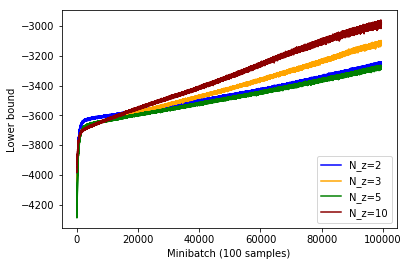
\includegraphics[width = 0.45\textwidth]{fig/gaussian-lb}
\caption{Variational Lower Bound implementing AEVB for Bernoulli case MNIST (left) and Gaussian case FreyFaces (right), with latent variable z of dimension 2, 3, 5 and 10.} \label{fig:VB-LB}
\end{center}
\end{figure}

Both models converge after sufficient epochs. The numerical result of lower bound is very similar to the paper we are replicating. Bernoulli case lower bound converges to around -150 and Gaussian case converges to around -3000. %Bernoulli $10^5$ epochs takes around 5 minutes on vm machine and Gaussian $10^6$ epochs takes around 30 minutes on vm, exact time is listed in comparative analysis and optimization section. 

Regarding the dimension of latent variable $z$, we find that higher dimension of latent variable results in a higher lower bound, and thus a closer approximation to true posteriors in both cases. Kingma and Welling (2013) pointed out in the original paper that superfluous latent variable did not result in overfitting because of the regularization nature of lower bound.

The marginal likelihoods are shown below, with similar shape and convergence to lower bounds and a higher accuracy with respect to higher dimension of $z$.

\begin{figure}[H]
\begin{center}
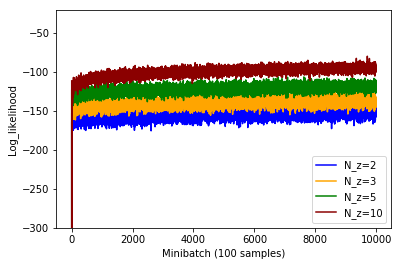
\includegraphics[width = 0.45\textwidth]{fig/Bernoulli_loglikelihood}
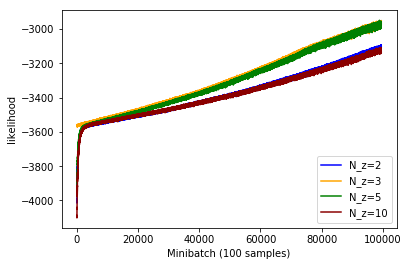
\includegraphics[width = 0.45\textwidth]{fig/gaussian-loglikelihood}
\caption{Marginal loglikelihood of original data $x$ implementing AEVB for Bernoulli case MNIST (left) and Gaussian case FreyFaces (right), with latent variable z of dimension 2, 3, 5 and 10. } \label{fig:VB-Likelihood}
\end{center}
\end{figure}


\subsection{Reconstruction and Visualization}
We use our trained model of learned parameter $theta$ and $\phi$ on our test set to reconstruct the test set data after compressing into a lower dimension space. We show an example of visualizing the test set reconstruction of MNIST and FreyFaces in 2D latent variable case. 

\begin{figure}[H]
\begin{center}
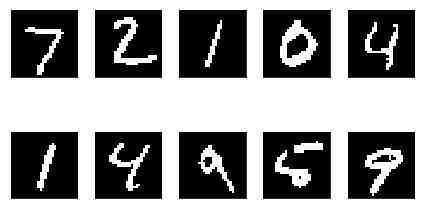
\includegraphics[width = 0.45\textwidth]{fig/Bernoulli_test}\\
\vspace{5mm}
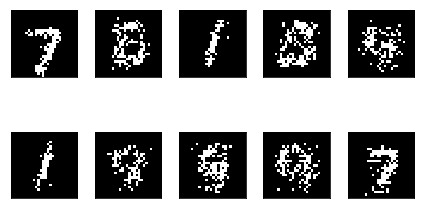
\includegraphics[width = 0.45\textwidth]{fig/Bernoulli_new}
\caption{MNIST using Bernoulli decoder AEVB with 2D latent variable z, first two lines are original test set example and the last two lines are the reconstruction result} \label{fig:MNIST-reconst}
\end{center}
\end{figure}

\begin{figure}[H]
\begin{center}
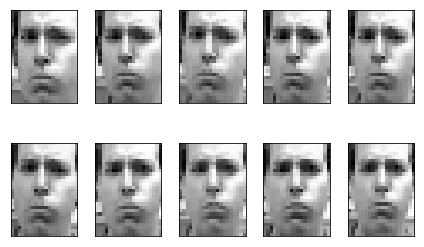
\includegraphics[width = 0.45\textwidth]{fig/f_test1}\\
\vspace{5mm}
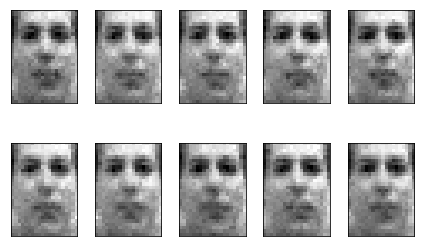
\includegraphics[width = 0.45\textwidth]{fig/f_new1}\\
\caption{FreyFaces using Gaussian decoder AEVB with 2D latent variable z, first two lines are original test set example and the last two lines are the reconstruction result} \label{fig:FreyFaces-reconst}
\end{center}
\end{figure}
\end{document}